General description of the proposed method

Definir segmentos

\subsection{Descripci\'on}\label{sec:method_description}

FILL ME


\subsection{Selecci\'on de muones y segmentos}\label{sec:selection}

FILL ME


\subsection{Muestra de simulaci\'on utilizada}\label{sec:sample}

Se han generado 100000 eventos de $Z'$ con $m_{Z'}$ = 5000 GeV fruto de la colisiones prot\'on-prot\'on a una energ\'ia de centro de masas de 13 TeV (condiciones del acelerador LHC) mediante simulaci\'on de Monte-Carlo utilizando el programa MadGraph5~\cite{Alwall:2014hca}. Se impone que las part\'iculas $Z'$ generadas se desintegren a un par de muones $\mu^{+}\mu^{-}$ y se simula el paso de los muones por el detector CMS con el paquete Geant4~\cite{Agostinelli:2002hh}. De esta manera se tiene una muestra con estad\'istica razonable de muones high-$p_{T}$ con $p_{T}$ generado conocido que se usar\'a para el entrenamiento de la DNN.

En la Figura~\ref{fig:data_pt} se muestran las distribuciones del $p_{T}$ generado y el $p_{T}$ proporcionado por el algoritmo TuneP de todos los muones de la muestra que pasan la selecci\'on detallada en la Secci\'on~\ref{sec:selection}.

\begin{figure}
\centering
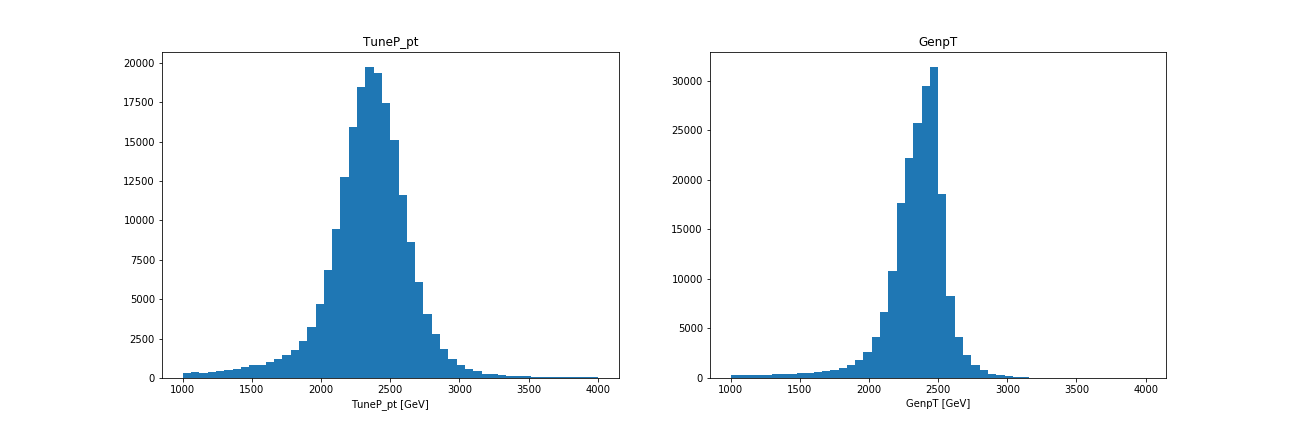
\includegraphics[width=0.60\textwidth]{figures/data_pt.png}
\caption{Distribuciones del momento transverso de los muones de la muestra de simulaci\'on utilizada. Izquierda: $p_{T}$ generado. Derecha: $p_{T}$ proporcionado por el algoritmo TuneP.}
\label{fig:data_pt}        
\end{figure}



